\documentclass[border=10pt]{standalone}

\usepackage{tikz}
\usepackage{tikzsymbols}
\usetikzlibrary{calc,patterns,shapes.geometric}

\def\centerarc[#1](#2)(#3:#4:#5){\draw[#1] ($(#2)+({#5*cos(#3)},{#5*sin(#3)})$) arc (#3:#4:#5);}

\begin{document}
	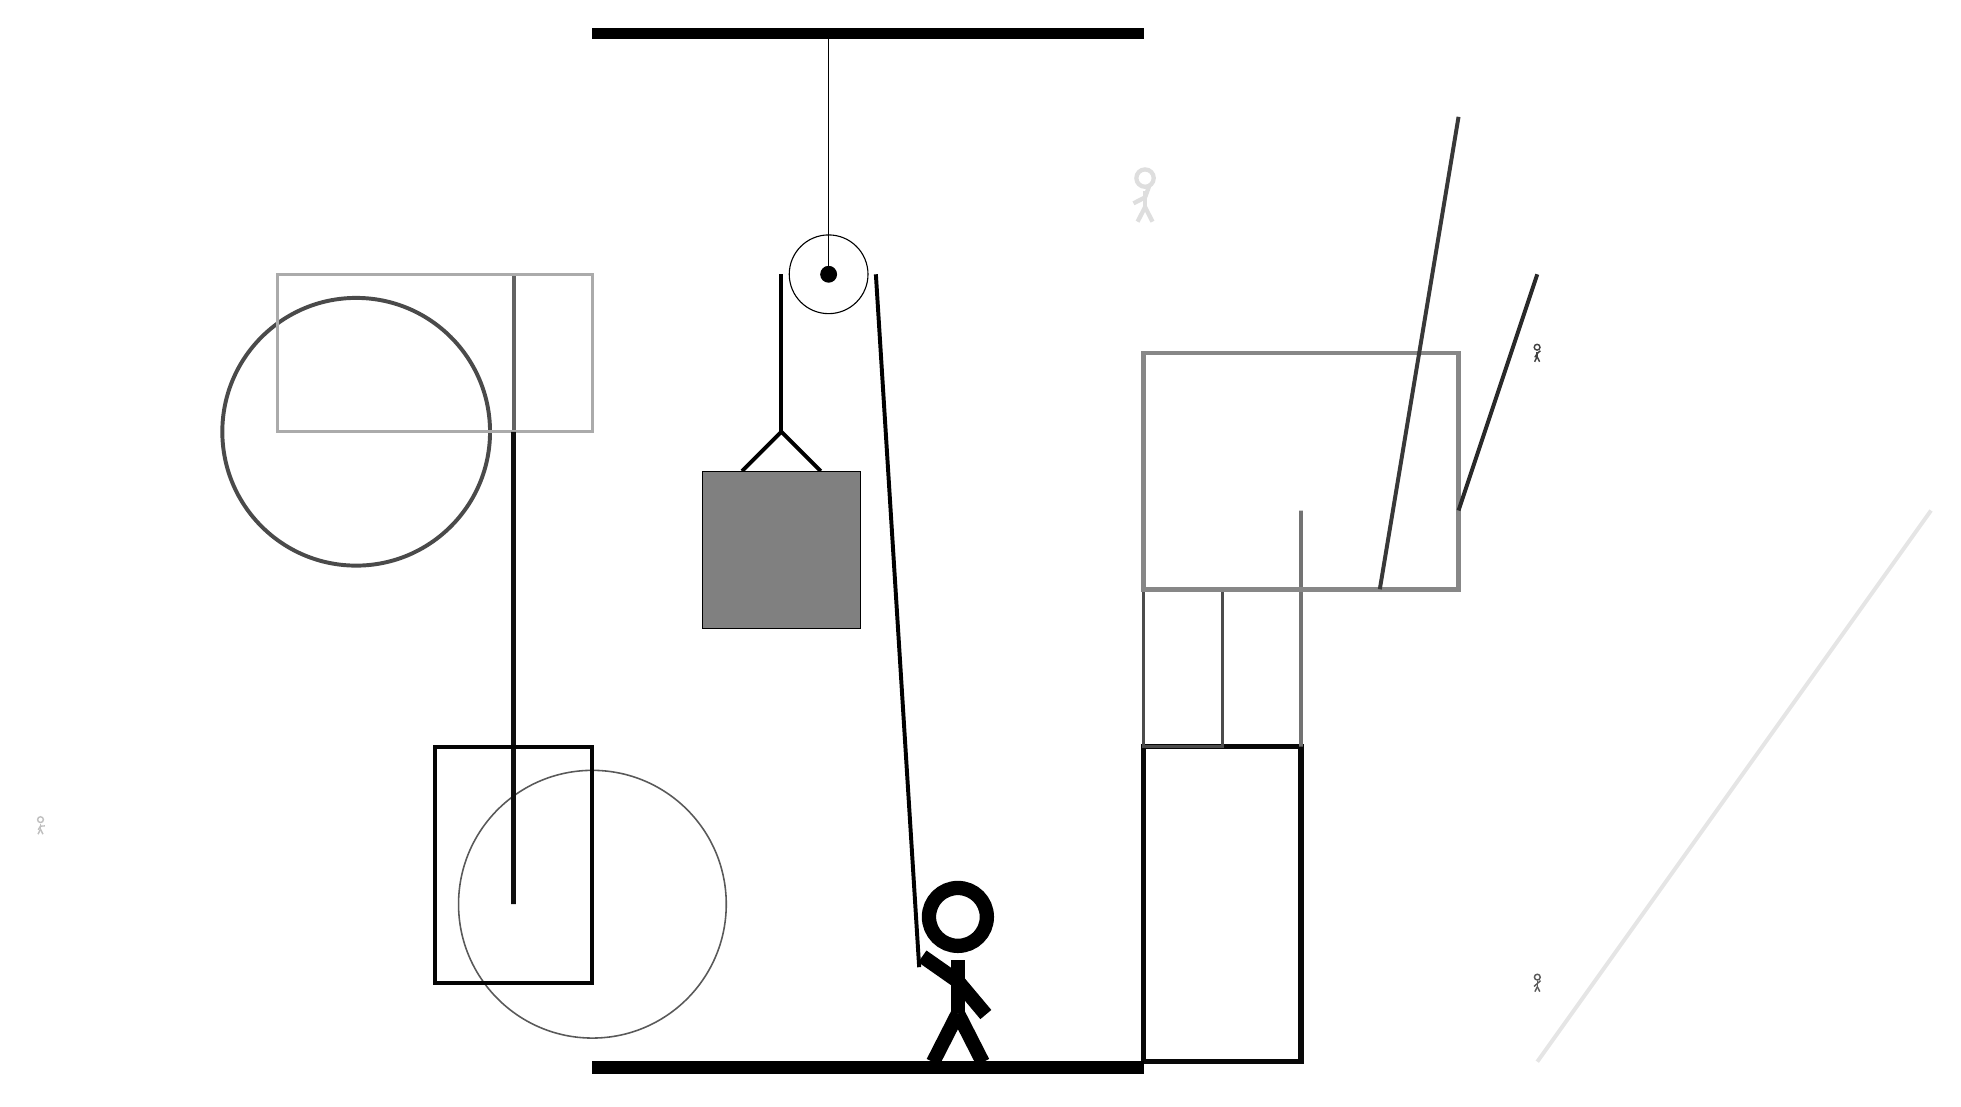
\begin{tikzpicture}
		%%%%% START %%%%%
		
		\draw[fill=black] (-2, 10) rectangle (5, 10.125);
		
		\draw (1, 7) circle (0.5);
		\draw[fill=black] (1, 7) circle (0.1);
		\draw (1, 10) -- (1, 7);
		
		\draw[line width=0.5mm] (-0.1, 4.5) -- (0.4, 5.0) -- (0.9, 4.5);
		\draw[fill=black!50] (-0.6, 4.5) rectangle (1.4, 2.5);
		
		\node[line width=0.6mm, color=black!13] at (5, 8) {\Strichmaxerl[3][27][70]};
		
		\draw[line width=0.7mm, color=black!97] (7, 1) rectangle (5, -3);
		\draw[line width=0.6mm, color=black!55] (7, 4) rectangle (7, 1);
		\draw[line width=0.5mm, color=black!72](9, 3) -- (6, 3);
		\draw[line width=0.4mm, color=black!70] (6, 1) rectangle (5, 3);
		
		\draw[line width=0.5mm, color=black!61](-3, 7) -- (-3, 3);
		\draw[line width=0.6mm, color=black!47] (5, 3) rectangle (9, 6);
		\node[line width=0.4mm, color=black!65] at (10, -2) {\Strichmaxerl[1][41][43]};
		\draw [line width=0.5mm, color=black!71](-5, 5) circle (1.7);
		\draw [line width=0.2mm, color=black!65](-2, -1) circle (1.7);
		\draw[line width=0.5mm, color=black!84](9, 4) -- (10, 7);
		\draw[line width=0.4mm, color=black!33] (-2, 5) rectangle (-6, 7);
		\node[line width=0.7mm, color=black!25] at (-9, 0) {\Strichmaxerl[1][59][2]};
		
		\draw[line width=0.7mm, color=black!94] (-3, 5) rectangle (-3, -1);
		\draw[line width=0.5mm, color=black!78](8, 3) -- (9, 9);
		\node[line width=0.3mm, color=black!75] at (10, 6) {\Strichmaxerl[1][58][42]};
		\draw[line width=0.5mm, color=black!98] (-2, 1) rectangle (-4, -2);
		\draw[line width=0.5mm, color=black!10](10, -3) -- (15, 4);
		
		\draw[line width=0.5mm] (0.4, 7) -- (0.4, 5.0);
		\centerarc[line width=0.5mm](1, 7)(0:180:0.6);
		\draw[line width=0.5mm](1.6, 7) -- (2.15, -1.8);
		
		\node at (2.6, -1.9) {\Strichmaxerl[10][-35][-50]};
		
		\draw[fill=black] (-2, -3) rectangle (5, -3.15);
		
		%%%%% END %%%%%
	\end{tikzpicture}
\end{document}